\documentclass[11pt]{article}
\usepackage[utf8x]{inputenc}
\usepackage{graphicx}
\usepackage{amsmath,amssymb}
\usepackage{textcomp}
\usepackage[total={6.5in,8in}]{geometry}
\usepackage{color}
\usepackage{natbib}
\bibliographystyle{abbrvnat}
\setcitestyle{authoryear,open={(},close={)}}
\usepackage{todonotes}

%%%%
\newcommand{\vf}[2][noinline]{\todo[#1, color=red!30!white]{\texttt{VF}: #2}}
\newcommand{\rtext}[1]{\textcolor{red}{#1}}
\newcommand{\parcial}[2]{\dfrac{\partial#1}{\partial#2}}
%%%%

\title{Reaction-diffusion model for the arrest of oscillations in the
	somitogenesis segmentation clock}

\author{Jes\'us Pantoja-Hern\'andez\textsuperscript{1}, V\'ictor F. Bre\~na-Medina\textsuperscript{2}, Mois\'es Santill\'an\textsuperscript{1}}

\date{\today}

\begin{document}
	\maketitle
	
	
\begin{enumerate}
\item Centro de Investigaci\'on y de Estudios Avanzados del IPN, Unidad Monterrey, Vía del Conocimiento 201, Parque PIIT, 66628 Apodaca NL, México.
\item Department of Mathematics, ITAM, Río Hondo 1, Ciudad de México 01080, México.
\end{enumerate}

	\begin{abstract}
	The clock and wavefront model is arguably the most widely accepted model for explaining the embryonic process of somitogenesis. According to this model, somitogenesis is based upon the interaction between a genetic oscillator, known as segmentation clock, and a moving wavefront, which provides the positional information indicating where each pair of somites is formed. Recently, \citet{Cotterell2015} reported a conceptually different mathematical model for somitogenesis. The authors called it a progressive oscillatory reaction-diffusion (PORD) model. In this model, somitogenesis is driven by short-range interactions and the posterior movement of the front is a local, emergent phenomenon, which is not controlled by global positional information. With the PORD model, it was possible to explain some experimental observations that are incompatible with the clock and wavefront model. However the PORD model has some important disadvantages of its own. Namely, it is quite sensitive to fluctuations and depends on very specific initial conditions (which are not biologically realistic). In this work, we propose a hybrid model, between the clock-and-wavefront and the PORD ones, and show that it able to overcome most of the inconveniences of the originating models.
	\end{abstract}
	
	\section{Introduction}
	\label{intro}
	
	Somitogenesis, the process by which somites are formed, is an essential
	developmental stage in many species. Somites are bilaterally paired blocks of
	mesoderm cells that form along the anterior-posterior axis of the developing
	embryo in segmented animals \citep{Maroto2012}. In vertebrates, somites give
	rise to skeletal muscle, cartilage, tendons, endothelial cells, and dermis.
	Somites form with a strikingly regular periodicity, that is preserved among
	embryos of a single species. From this, and other reasons, scientists have been
	attracted to somitogenesis for decades. One of the earliest conceptual attempts
	to explain this regularity is the so-called clock and wavefront model,
	originally proposed by \citet{Cooke1976}. According to this model, somitogenesis
	occurs due to the interaction between: (i) autonomous oscillations of a network
	of genes and gene products, which causes presomitic-mesoderm cells to oscillate
	between a permissive and a non-permissive state, in a consistently (clock-like)
	timed fashion; and (ii) a wavefront (also known as determination front) of
	signaling that slowly progresses in an anterior-to-posterior direction. As the
	wavefront comes in contact with cells in the permissive state, they undergo a
	mesenchymal-epithelial transition, forming a somite boundary, and resetting the
	process for the next somite.
	
	The clock and wavefront model gained relevance when the expression of several
	genes under the Notch, Wnt, and FGF pathways was discovered to oscillate
	cyclically, with the same period as that of somite formation
	\citep{Palmeirim1997, Pourquie2001, Gibb2010, Pourquie2011}. This, together with
	the existence of substances, like Wnt3a and FGF8, whose concentrations
	vary along the presomitic mesoderm in characteristic patterns that travel at
	constant velocity in an anterior to posterior direction, seemed to confirm the
	general assessments of the clock and wavefront model \citep{Dubrulle2001,
		Gibb2010, Pourquie2011}. As a matter of fact, this model has been so
	successful because it agrees with numerous experimental observations, and
	because much progress has been done in elucidating the segmentation-clock
	clockwork, and the way it interacts with the Wnt3a and FGF8 gradients.
	Despite its success, some experimental observations have been reported that are
	incompatible with the clock and wavefront paradigm. For instance, somites can
	form in the absence of Wnt or FGF gradients, albeit in a disorderly
	fashion \citep{Naiche2011,Dias2014}.
	
	Recently, \citet{Cotterell2015} introduced a novel mathematical model for
	somitogenesis. Contrarily to the clock and wavefront model, in the model by
	\citeauthor{Cotterell2015}---which the authors call a progressive oscillatory
	reaction-diffusion (PORD) system---somitogenesis is driven by short-range
	interactions. Hence, the posterior movement of the front is a local, emergent
	phenomenon, that is not controlled by global positional information. As shown by
	\citeauthor{Cotterell2015}, their PORD model is compatible with several
	important features of somitogenesis (like size regulation), that former
	reaction-diffusion models were unable to explain. Furthermore, the PORD model
	makes predictions regarding FGF-inhibition and tissue-cutting experiments that
	are more consistent with experimental observations than those of clock and
	wavefront models.
	
	\begin{figure}[t!]
		\centering
		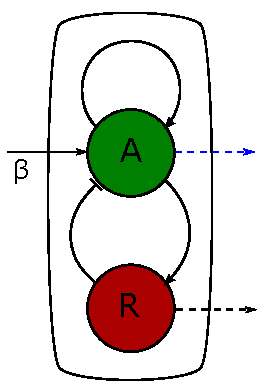
\includegraphics[width=2in]{Figures/Fig01.pdf}
		\caption{Schematic representation of the gene regulatory network introduced by
			\citep{Cotterell2015} and studied in the present work. This network consists of
			two genes: an activator \textit{A} and a repressor \textit{R}. Solid lines
			ending in arrowheads (hammerheads) denote positive (negative) regulation.
			$\beta$ represents external regulation of gene \textit{A} via a wavefront
			substance. Dashed lines correspond to passive diffusion into the extracellular
			medium. The diffusion process depicted by the blue arrow was not
			originally included in the \citeauthor{Cotterell2015} model, but is 
			included in the modified model version studied in this work.}
		\label{Fig01}
	\end{figure}
	
	At the core of the \citeauthor{Cotterell2015} model there is a gene regulatory
	motif schematically depicted in Fig. \ref{Fig01}. In this network, a
	hypothetical gene codes for an activator protein (A), which enhances its own
	expression, as well as that of another gene that codes for a hypothetical
	repressor protein (R). In turn, the repressor protein down-regulates the gene
	coding for the activator, and is able to diffuse into the extracellular medium
	and affect neighboring cells. \citeauthor{Cotterell2015} did not identify the
	network genes, but showed that in case it existed, the gene network in Fig.
	\ref{Fig01} can explain most of the experimental observations regarding
	somitogenesis. In particular, with the correct parameter values, such gene
	network can generate sustained oscillations, and when repressor diffusion is
	included, it gives rise to a stationary pattern of gene expression like that
	observed in somitogenesis, even in the absence of a FGF wavefront.
	
	Even though the hypothetical genes in the \citeauthor{Cotterell2015} model have
	not been identified, we find this model interesting for the following reasons:
	(i) as far as we have observed, it accounts for some important features of
	somitogenesis that traditional clock and wavefront models fail to explain; (ii)
	a gene network with a similar architecture as that of Fig. \ref{Fig01}---albeit
	with a different dynamic behavior---has been invoked to explain oscillation
	arrest in somitogenesis \citep{Santillan2008, Zavala2012}; and finally, (iii)
	the architecture of the gene network in Fig. \ref{Fig01} is an ubiquitous motif
	in the intricate transcription-factor regulatory network of the genes under the
	Wnt, Notch and FGF pathways \citep{Gibb2010, Zavala2012}.
	
	In opposition to its multiple virtues, the \citeauthor{Cotterell2015} model is
	quite sensitive to fluctuations. For instance, when random perturbations of
	initial conditions or intrinsic noise are present, a disordered pattern of gene
	expression arises. This behavior resembles what happens with PSM cells that are
	not under the influence of a wavefront, but contrasts with the observed
	robustness of somite formation under normal conditions. Another important issue 
	of the \citeauthor{Cotterell2015} model is that it requires very specific initial
	conditions (which are not biologically realistic) 
	to give rise to a segmentation pattern. We hypothesize from the
	above discussion that, although a wavefront is not strictly necessary for the
	\citeauthor{Cotterell2015} model to generate a gene expression pattern
	consistent with somitogenesis, the interaction with a wavefront is essential to
	explain the observed robustness of this phenomenon and to eliminate the dependence
	on specific initial conditions. In other words, we argue 
	that a hybrid model that accounts for the diffusion of the regulatory substances
	(as in the PORD model), as well as for a global wavefront that interacts
	with the oscillatory gene network (as in the clock and wavefront paradigm), 
	may circumvent the disadvantages of the original models. The present work is aimed at
	testing this hypothesis, and discussing the corresponding biological
	implications.
	
	The manuscript is organized as follows. In section 2 we develop a hybrid
	model between the PORD and the clock-and-wavefront models. In section 3 we 
	define the parameter set where the dynamics of the non-diffusion system give place 
	to a limit cycle family. In section 4 we explain the numerical methods used as 
	well as the initial and boundary conditions. In section 5 we show results of the
	simulations for each one of the selected conditions. Finally, we discuss the 
	relevance of the results obtained as well as the limitations of the model in 
	section 6.
	
	\section{Mathematical Model}
	\label{model}
	
	In this section, we introduce a modified version of the
	\citeauthor{Cotterell2015} model. As the functions taken into account in the
	original model are unrealistic from a biochemical point of view, we propose key
	modifications, which consist in replacing the gene-expression regulatory
	functions and introducing a diffusion transport process for both activator and
	repressor protein concentrations.
	
	Consider the gene network schematically represented in Fig. \ref{Fig01}. Assume
	that the half life of mRNA molecules corresponding to genes \textit{A} and
	\textit{R} is much shorter than that of the corresponding proteins. Then, a
	quasi-stationary approximation can be made for the equations governing mRNA
	dynamics, which yields the following reaction-diffusion system for the concentration of
	proteins $A$ and $R$:
	\begin{subequations}\label{eq012}
		\begin{flalign}
		& \frac{\partial A}{\partial t} = \alpha_A P_A (A, R) - \mu_A A + D_A \nabla^2 A\,,
		\label{eq01} \\
		& \frac{\partial R}{\partial t} = \alpha_R P_R (A) - \mu_R R + D_R \nabla^2 R\,,
		\label{eq02}
		\end{flalign}
	\end{subequations}
	where $\alpha_A$ and $\alpha_R$ are the maximum possible rate of activator and
	repressor production; $P_A$ and $P_B$ are the probabilities that the promoters
	of genes $A$ and $R$ are active; degradation rate constants of each protein
	concentration are denoted by $\mu_A$ and $\mu_R$, respectively; and $D_A$ and
	$D_R$ are the corresponding diffusion coefficients.
	
	To take into account the roles of the activator and the repressor, $P_A(A, R)$
	must be a monotonic increasing (decreasing) function of $A$ ($R$), while
	$P_R(A)$ ought to be a monotonic increasing function of $A$. Indeed,
	\citet{Cotterell2015} proposed the following functions:
	\begin{subequations}\label{eq034}
		\begin{gather}
		P_A(A, R) = \displaystyle \Phi \left(
		\frac{l_1 A - l_2 R + \beta}{1 + l_1 A - l_2 R + \beta}
		\right), \label{eq03} \\[3mm]
		P_R(A) = \displaystyle \frac{l_3 A}{1 + l_3 A}, \label{eq04}
		\end{gather}
	\end{subequations}
	where $l_1$, $l_2$, and $l_3$ define the strengths of regulatory interactions
	between \textit{A} and \textit{R}, and $\beta$ is the background regulatory
	input of \textit{A}. To prevent negative values, \citeauthor{Cotterell2015}
	introduced the function $\Phi(x) = x.H(x)$, where $H(x)$ is the standard
	Heaviside function ($H(x) = 1$ for $x \geq 0$ and $H(x) = 0$ for $x < 0$).
	
	Even though the function $P_A(A, R)$ defined in (\ref{eq03}) fulfills the
	requirement of being a monotonic decreasing function of $R$ and a monotonic
	increasing function of $A$, it shows features that are biologically challenging:
	\begin{itemize}
		\item There is neither biological nor biochemical motivation for the introduction of function
		$\Phi$.
		\item Function $\Phi(x)$ is non smooth at the origin. This feature is
		unusual in biologically inspired mathematical models, and may cause unexpected
		complications while studying the dynamical system.
		\item Since the term $l_2 R$ appears with negative sign in the denominator of
		the argument of function $\Phi$, in the right hand side of Eq. (\ref{eq03}),
		function $P_A(A, R)$ may be divergent for certain values of $A$ and $R$.
	\end{itemize}
	
	In order to address the above discussed issues, we propose a slightly novel approach by
	substituting the promoter-activation probabilities in \eqref{eq034} with functions that are consistent
	with the assumptions that the activator and the repressor compete for
	the same binding site in the promoter region of gene $A$, and that both the
	activator and the repressor interact with their corresponding binding sites in
	the promoter regions of genes $A$ and $R$ in a cooperative fashion
	\citep{Santillan2008b}. In so doing, we have
	\begin{subequations}\label{eq056}
		\begin{gather}
		P_A(A,R) = \displaystyle \frac{\beta + (A/K_1)^{n_1}}{1 + (A/K_1)^{n_2} +
			(R/K_2)^{n_2}}\,, \label{eq05} \\[3mm]
		P_R(A)  = \displaystyle \frac{(A/K_3)^{n_3}}{1 + (A/K_3)^{n_3}}\,,
		\label{eq06}
		\end{gather}
	\end{subequations}
	where $K_1$ denotes the half saturation constant for the binding reaction
	between the activator and the promoter of gene $A$; the Hill coefficient that
	accounts for a cooperative interaction between the activator and gene $A$
	promoter is given by $n_1$; as in the original model, $\beta$ is the background
	regulatory input of $A$; the half saturation constant and Hill coefficient of
	the interaction between the repressor and the promoter of gene $A$ are
	represented by $K_2$ and $n_2$, respectively; and $K_3$ and $n_3$, equivalently,
	are the half saturation constant and Hill coefficient for the interaction
	between the activator and the promoter of gene $R$. 
	
	Notice that \eqref{eq012} along with \eqref{eq056} constitute a
	reaction-diffusion system for the gene expression network depicted in
	Fig.~\ref{Fig01}, which accounts for spatio-temporal interactions between these
	two protein concentrations.
	
	Upon re-scaling position and time as $x' = x / L$, $y' = y / L$, $z' = z / L$,
	and $t' = t \mu_A$ and substituting the following dimensionless variables and
	parameters 
	\begin{gather*}
	a  =  \dfrac{A \mu_A}{\alpha_A},  \qquad  d_a  =  \dfrac{D_A}{ \mu_A L^2}, 
	\qquad k_1  =  \dfrac{K_1 \mu_A }{ \alpha_1},  \qquad k_2  =  \dfrac{K_2 \mu_R
	}{\alpha_3},  \\
	r  =  \dfrac{B \mu_r }{ \alpha_r}, \qquad  d_r  = \dfrac{ D_R }{ \mu_A L^2},
	\qquad k_3  =  \dfrac{K_3 \mu_R }{ \alpha_R},  \qquad  \mu  = \dfrac{ \mu_R 
	}{\mu_A}, 
	\end{gather*}
	where $L$ is a characteristic length on system \eqref{eq012}-\eqref{eq056}, we
	obtain the reaction-diffusion system in a dimensionless form 
	\begin{subequations}\label{eq078910}
		\begin{gather}
		\frac{\partial a}{\partial t'} =  P_a(a, r) - a + d_a \nabla'^2 a, \label{eq07} \\
		\frac{\partial r}{\partial t'}  =  \mu\left (P_r(a) - r + d_r \nabla'^2 r\right),
		\label{eq08}
		\end{gather}
		where $\nabla'$ is the Laplacian with respect to $(x', y', z')$, and
		\begin{gather}
		P_a(a, r)  =  \displaystyle \frac{\beta + (a / k_1)^{n_1}}{1 + (a /
			k_1)^{n_1} + (r / k_2)^{n_2}}, \label{eq09} \\[2mm]
		P_r(a)  =  \frac{(a / k_3)^{n_3}}{1 + (a / k_3)^{n_3}}. \label{eq10}
		\end{gather}
	\end{subequations}
	To ease notation, we suppress symbol $(\cdot)^\prime$ from this point onward
	along the paper.
	
	\section{Parameter estimation}
	\label{param}
	
	Since the genes here modeled are hypothetical, it is impossible to estimate the
	model parameter values from experimental data. Instead, we performed a
	bifurcation analysis of the system with no diffusion ($d_a = d_r = 0$),
	employing a continuation method implemented in \texttt{XPPAUT}
	\citep{Ermentrout1987}. The results of this analysis are presented in
	Fig.~\ref{FigA01} of Appendix \ref{app:bif}. From this analysis, we determined
	the parameter intervals (see Table \ref{Tab01}) for which the system shows
	sustained oscillations in the absence of diffusion, which is crucial to set the
	periodicity of somitogenesis. In our simulations, we consider parameter values in
	the middle of the intervals reported in Table \ref{Tab01}. Following
	\citep{Cotterell2015}, we fixed $n_3 = \mu = 1$, and assumed that $n = n_1 =
	n_2$. After this, the only free parameters in the model are the diffusion
	coefficients. 
	
	\begin{table}[h] 
		\centering
		\begin{tabular}{|c|} \hline
			$k_1  \in [0.029, 0.057]$ \\ \hline
			$k_2  \in [0.008, 0.017]$ \\ \hline 
			$k_3  \in [1.658, 3.642]$ \\ \hline
			$n  \in  [2.411, 5.025]$ \\  \hline
			$\beta  \in  (0, 2.25]$ \\   \hline
		\end{tabular} 
		
		\caption{Parameter intervals for which the system with no diffusion shows
			sustained stable oscillatory behavior.}
		\label{Tab01}
	\end{table}
	
	\section{Numerical methods}
	\label{numer}
	
	Under the supposition that the presomitic mesoderm (PSM) can be regarded as
	one-dimensional, we considered a single spacial dimension, $x$, with boundaries
	at $x=0$ and $x=1$. These boundaries set an observation window in the PSM, where
	$x=0$ corresponds to the posterior extreme. To numerically solve
	system~\eqref{eq078910}, we implemented a standard finite-difference three-point
	stencil and Euler's algorithm in \texttt{Julia}; homogeneous Neumann boundary
	conditions were included:
	\begin{gather}\label{eqbn}
	\left. \dfrac{\partial a}{\partial x}\right|_{(0, t)} = 
	\left. \dfrac{\partial a}{\partial x}\right|_{(1, t)} = 
	\left. \dfrac{\partial r}{\partial x}\right|_{(0, t)} =
	\left. \dfrac{\partial r}{\partial x}\right|_{(1, t)} = 0 ,
	\end{gather}
		
	We also performed stochastic simulations in which additive white noise was added
	to the system. For these simulations we substituted equations \eqref{eq07} and
	\eqref{eq08} by
	\begin{subequations}\label{eq1112}
		\begin{gather}
		\frac{\partial a}{dt} = P_a(a, r) - a + d_a \nabla^2 a + c_v \overline{a} \,
		dW, \label{eq11} \\
		\frac{\partial r}{dt}= \mu (P_r(a) + r - d_r \nabla^2 r) + c_v \overline{r} \,
		dW, \label{eq12}
		\end{gather}
	\end{subequations}
	where $\overline{a}$ and $\overline{r}$ respectively denote the stationary
	values of  $a$ and $r$, $c_v$ is the coefficient of variation of the added white
	noise, and $dW$ is a normally-distributed white noise term with mean zero and
	variance 1. To solve this system of stochastic partial differential equations we
	employed the Euler-Maruyama method, implemented in \texttt{Julia}.
	
	We employed different initial conditions along the present work and so, they are specified before every simulation.

	\section{Results}
	\label{res}
	
	We started by reproducing the results in \citep{Cotterell2015}. To this end, we
	set $d_a=0$, $d_r = 2.5\times10^{-3}$, $\beta = 0.5$, and numerically solved the
	model equations as described in Section \ref{numer}, with the following initial 
	conditions:
	\begin{gather}
	a(x, 0) = \left\{\begin{array}{cl}
	0.05 & \text{for } x = 1, \\
	0 & \text{for } 0 \leq x < 1,
	\end{array} \right. 
	\quad
	r(x, 0) = 0, \; \text{for } 0 \leq x \leq 1\,.
	\end{gather}
	That is, the system is assumed to be initially homogeneous, except for a
	perturbation at the anterior extreme of the observation window.	
	The simulation results are
	shown in Fig.~\ref{Fig02}A. Observe that an oscillatory behavior
	gradually gives rise to a steady pattern consisting of alternated high and low
	gene-expression regions. Notice as well that the pattern formation dynamics start at
	the initial perturbation position, and propagate with constant speed. The
	initial perturbation is essential for the appearance of the pattern. If the
	system is initially homogeneous, the oscillatory behavior continues
	indefinitely---see Fig.~\ref{Fig02}B. On the other hand, when more than one
	initial perturbations are present, each one of them originates a
	pattern-formation wave, and when two such waves collide, they cancel out---see 
	Fig.~\ref{Fig02}C. These results suggest that the transition from an
	oscillatory behavior to a steady pattern of gene expression is due to a
	diffusion driven instability interacting with a limit cycle. To verify this,
	we investigated the spatial stability of the dynamical system
	in~\eqref{eq078910} and~\eqref{eqbn} in
	Appendix \ref{app:bif}. We were able to confirm
	that the limit cycle is unstable with the current parameter values set; see
	Fig.~\ref{FigB02}, panel (c), at $\kappa^2=0$.
	
	\begin{figure}[t!]
		\centering
		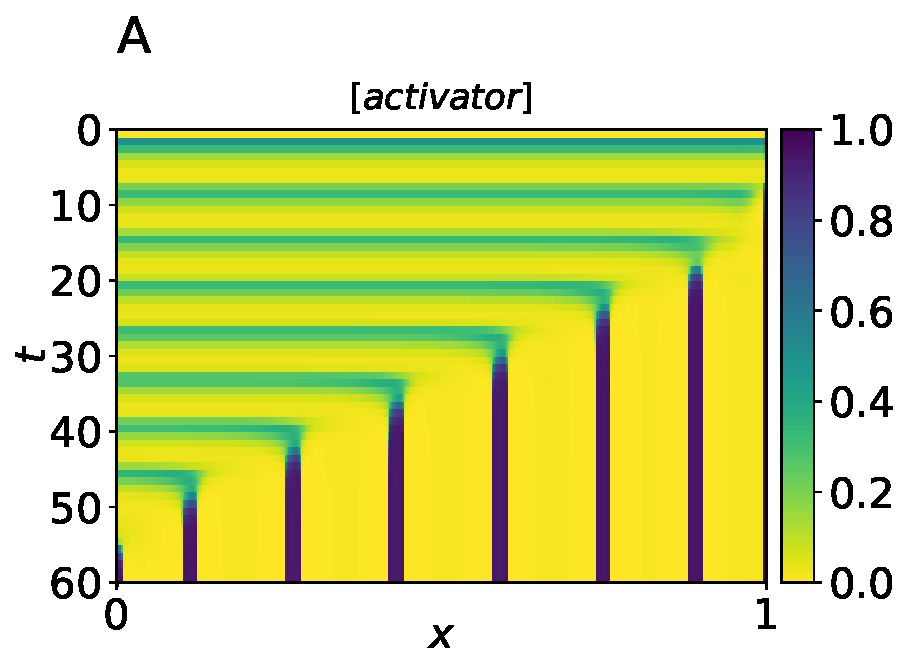
\includegraphics[width=2in]{Figures/Fig02aRev.pdf}
		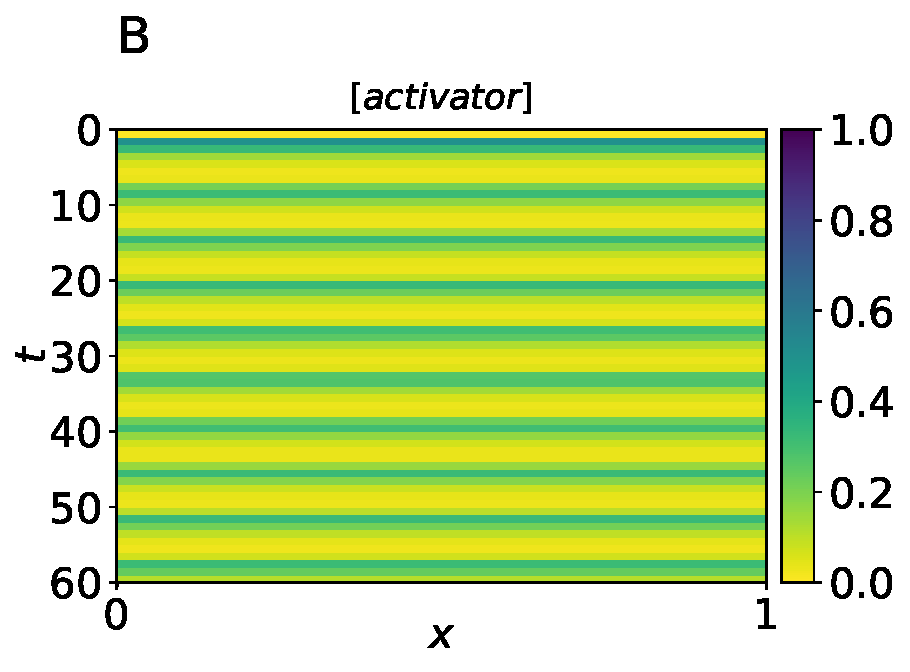
\includegraphics[width=2in]{Figures/Fig02bRev.pdf}
		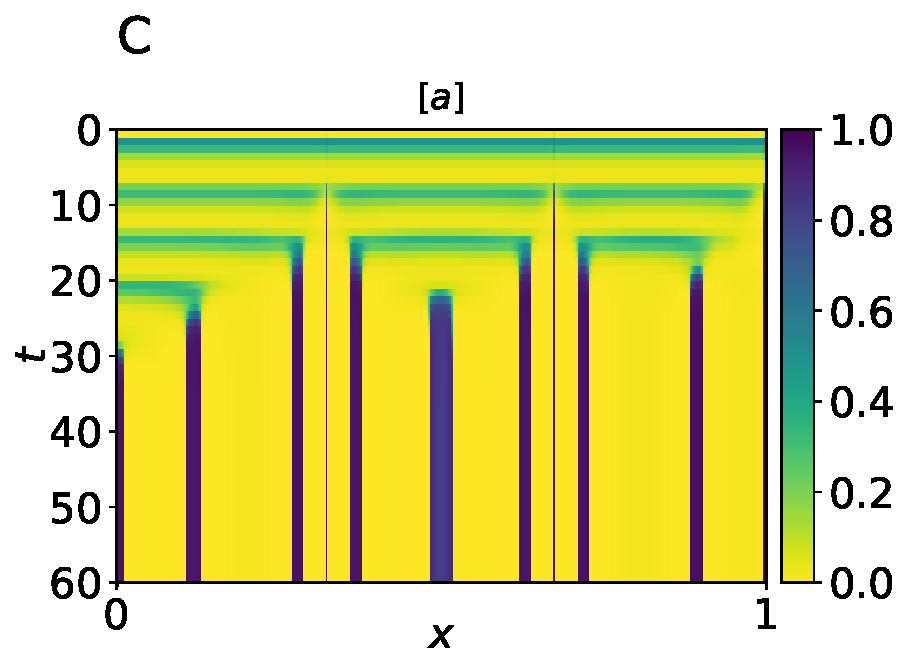
\includegraphics[width=2in]{Figures/Fig02cRev.pdf}
		\caption{Spatio-temporal evolution of $a$ from system~\eqref{eq078910}, with
			boundary condition as in~\eqref{eqbn}, for different initial conditions: (A)
			$r(x, 0)=0$ for all $x\in[0,1]$, $a(x, 0)=0$ for $0\leq x<1$, and $a(1, t) =
			0.05$; (B) $r(x, 0) = a(x, 0)=0$ for all $x\in[0,1]$; (C) $r(x, 0)=0$ and $a(x,
			0)=0$ for all $x\in[0,1]$ and $a(x',0)=0.05$ at $x'=0.325, 0.675, 0.9975$.
			Parameter values were set as follows: $k_1=0.05$, $k_2=0.01$, $k_3=2$, $n=3$,
			$\beta=0.5$, $d_a=0$, and $d_r=2.5\times10^{-3}$.}
		\label{Fig02}
	\end{figure}
	
	The results described in the previous paragraph are consistent with the reported
	experimental observations that somites can form in the absence of a wavefront
	(recall that somite formation 
	in the absence of a wavefront is incompatible with the clock and wavefront paradigm).
	As a matter of fact, they may explain why somites form almost simultaneously and
	irregularly; i.e. any initial perturbation in the mesoderm tissue would
	rapidly originate a somite boundary, and the emerging pattern formation wave would
	almost immediately collide with neighboring waves. 
	On the other hand, even though a wavefront is not strictly necessary for the 
	formation of somites, there are several reports that confirm its importance
	\citep{Sawada2001, Naiche2011} . In particular, the regularity of somite
	formation has been demonstrated to be extremely robust to many different kinds
	of perturbations on both the mesoderm tissue and the differentiation wavefront,
	and this robustness cannot be explained by PORD models. Moreover, PORD 
	models demand very specific initial conditions to produce ordered 
	segmentation patterns, but this is not biologically realistic.
	
	We hypothesize that somitogenesis robustness can be achieved via the interaction
	between the gene network and a wavefront, and that this will also eliminate 
	the stringent dependence on a specific initial condition. This wavefront is originated by 
	substances, like FGF8 (in what follows we refer to FGF8 only, but the
	discussion applies to other substances as well, like Wnt3a), which are produced in the
	embryo tail bud and diffuse to the rest of the PSM. In consequence, FGF8
	concentration decreases in the posterior to anterior direction. Furthermore, 
	as the embryo grows, the tail bud recedes leaving PSM cells behind. Hence,
	the spatial FGF8 distribution moves in the anterior to posterior direction, like
	a wavefront, as time passes. In other words, we expect that a stable limit cycle 
	emerges for large
	enough values of $\beta$ (that accounts for the PSM interaction with the
	wavefront), which maintains an oscillatory gene expression despite perturbations, 
	thus preventing somite formation close to the tail bud. Furthermore, if the limit
	cycle turns unstable below a given $\beta$ threshold, any local inhomogeneity would
	lead to the formation of a somite at the PSM position where the threshold is
	reached. This dynamic behavior may explain why somites are formed in an
	irregular fashion in the absence of FGF8, and how a FGF8 wavefront robustly
	drives somitogenesis.
	
	\begin{figure}[t!]
		\centering
		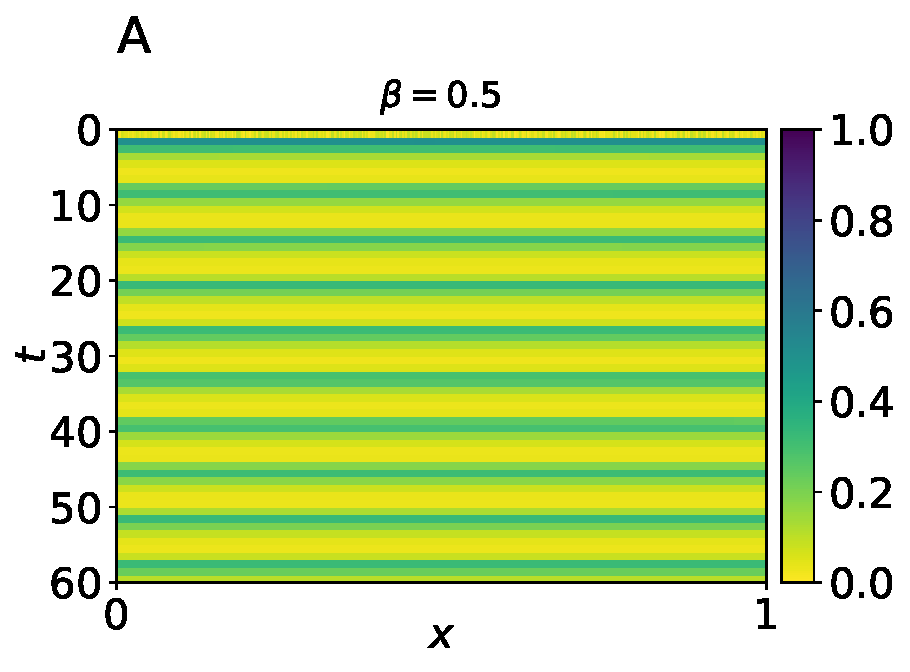
\includegraphics[width=2in]{Figures/Fig03aRev.pdf}
		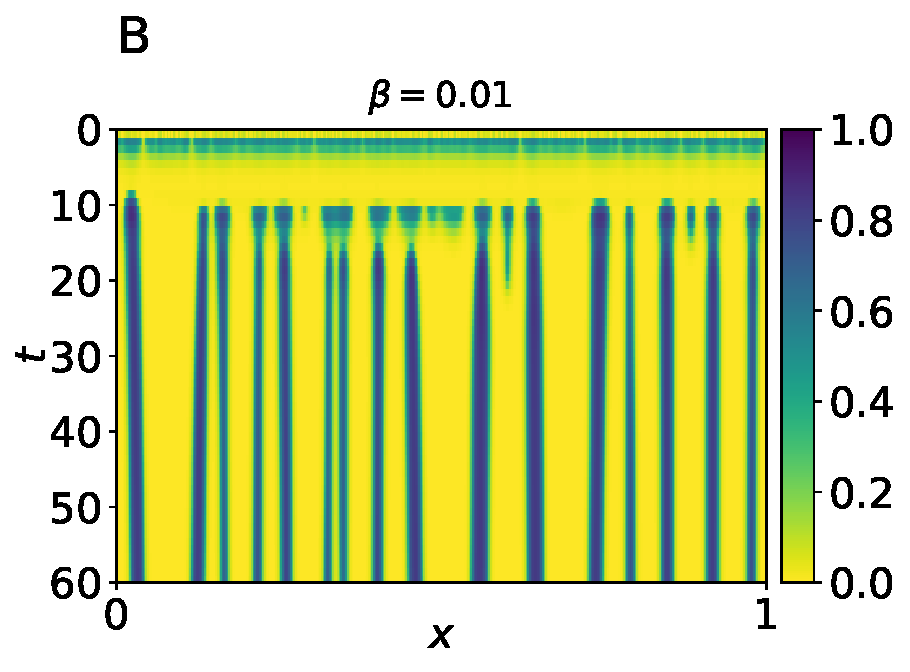
\includegraphics[width=2in]{Figures/Fig03bRev.pdf}
		\caption{Spatio-temporal evolution of $a$ from system~\eqref{eq078910}, with
			boundary condition as in~\eqref{eqbn}, for: (A) spatially stable with
			$\beta=0.5$; (B) spatially unstable with $\beta=0.01$. In both cases, the
			initial conditions for $a$ were selected from random uniform distributions in
			the interval $[0, 0.1]$, whereas we set $r(x, 0) = 0$ for all $x\in[0,1]$.
			Parameter values were set as follows: $k_1=0.05$, $k_2=0.01$, $k_3=2$, $n=3$, $d_a =
			5\times10^{-5}$ and $d_r=2.5\times10^{-3}$.}
		\label{Fig03}
	\end{figure}
	
	\begin{figure}[t!]
		\centering
		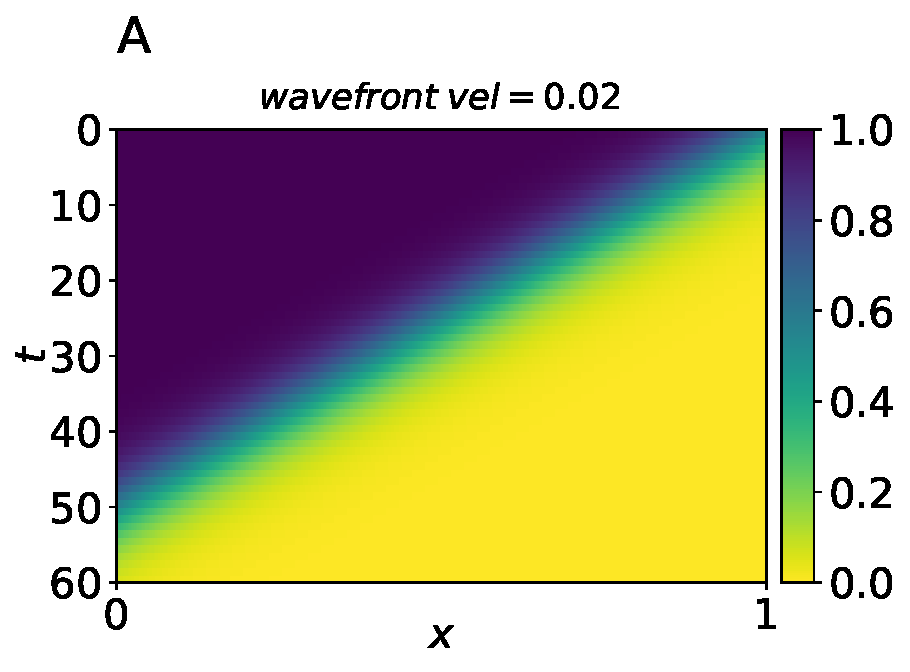
\includegraphics[width=2in]{Figures/Fig04aRev.pdf}
		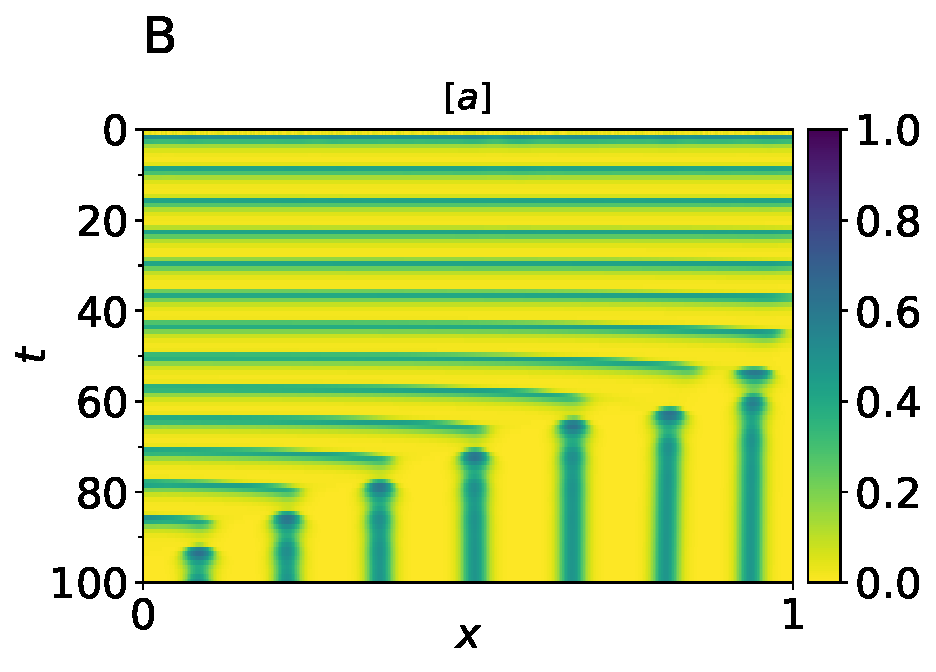
\includegraphics[width=2in]{Figures/Fig04bRev.pdf} \\
		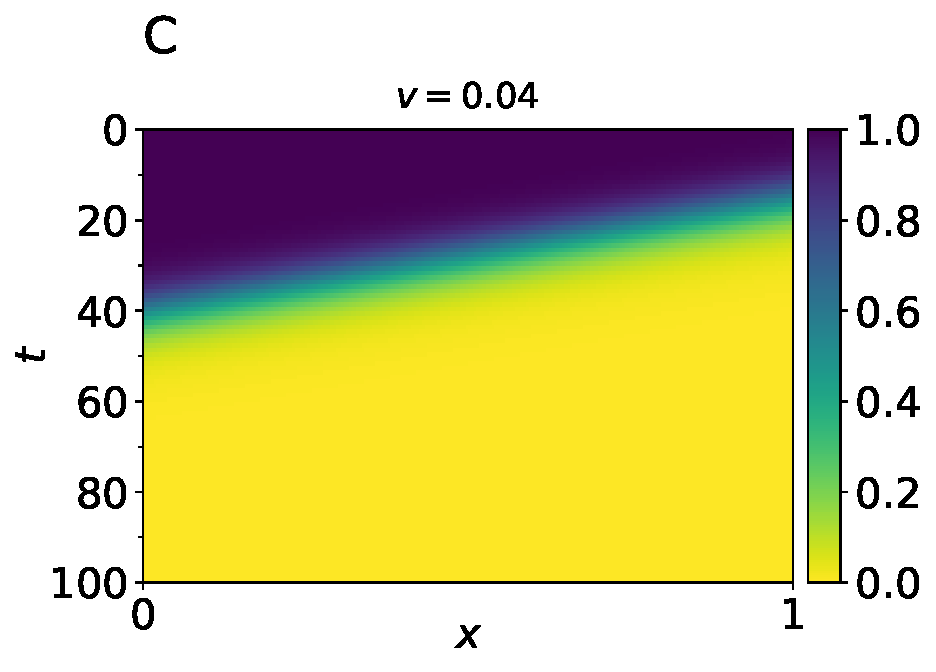
\includegraphics[width=2in]{Figures/Fig04cRev.pdf}
		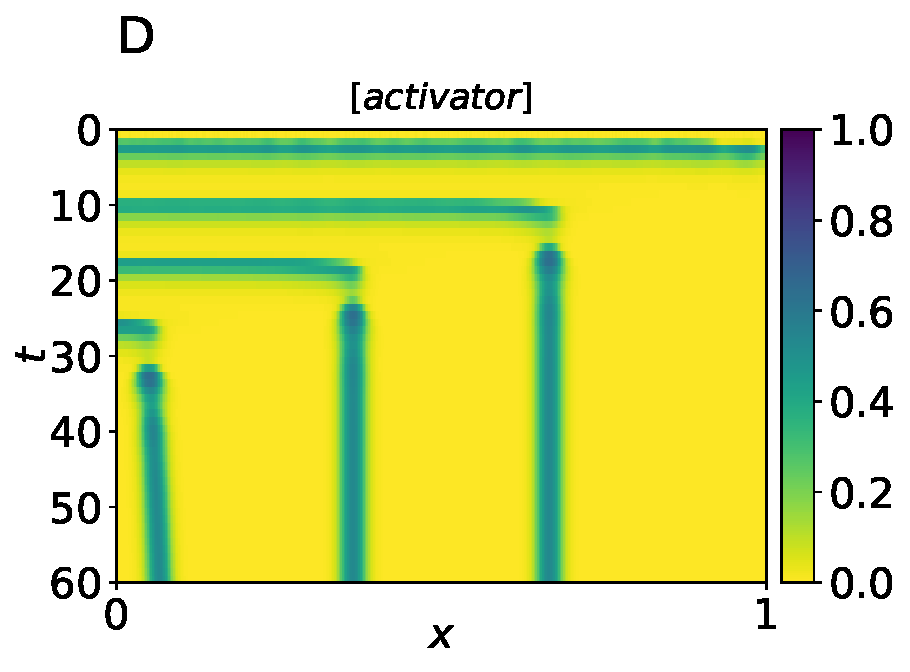
\includegraphics[width=2in]{Figures/Fig04dRev.pdf}
		\caption{Spatio-temporal evolution of $a$ from system~\eqref{eq078910} for
			$\beta$-wave speed as in~\eqref{eqbeta}, with boundary condition as
			in~\eqref{eqbn}. (A) $\beta$-wave evolution and (B) somite-pattern formation for
			speed $v=0.02$; (C)~$\beta$-wave evolution and (D) somite-pattern formation for
			speed  $v=0.04$. Initial conditions for~$a$ consists of random uniform
			distributions in the interval $[0, 0.1]$, whereas $r(x, 0) = 0$ for all
			$x\in[0,1]$. Parameter values were set as follows: $k_1=0.05$, $k_2=0.01$, $k_3=2$,
			$n=3$, $d_a = 5\times10^{-5}$ and~$d_r=2.5\times10^{-3}$.}
		\label{Fig04}
	\end{figure}
	
	In Appendix, \ref{app:bif} we analyze the stability of the PDE system when 
	depending of $\beta$ and $d_a$ parameters, and found that for a fixed value 
	for $d_a=5\times10^{-5}$ the system undergoes a bifurcation	from a stable to 
	an unstable limit cycle as the value of $\beta$ decreases. To illustrate these 
	findings, we present in Fig.~\ref{Fig03} the results of two
	simulations: one in which the limit cycle is stable and another in which it is
	unstable. In Fig.~\ref{Fig04} we present the results of two more runs where,
	instead of considering a constant value of~$\beta$, we assume that it is given
	by 
	\begin{gather}\label{eqbeta}
	\beta(x, t) = \beta_0 \frac{K^m}{K^m + (x - v t)^m}\,.
	\end{gather}
	Notice that this expression corresponds to a external regulation of gene A, which 
	is a temporarily and spatially dependent profile that decays in a sigmoidal 
	fashion in the posterior to anterior direction, and travels with speed
	$v>0$ in the opposite direction. That is, it mimics the behavior of the FGF8
	profile. For the simulations in Fig.~\ref{Fig04} we set $K =0.9 $, $m = 4 $
	(these values were also employed for the simulation in Fig.~\ref{Fig05}), and
	considered two different speed values $v = 0.02 $, and $v = 0.04$. Observe that, in
	both simulations, the pattern formation waves have the same periodicity, but the
	regions corresponding somites are larger for the faster wave. This result agrees
	with the experimental observation that somites are	larger when the velocity of 
	FGF8 profile is increased \citep{Sawada2001}. Interestingly, we did not have to 
	assume a specific initial condition for the correct segmentation pattern to arise.
	The simulations in Fig.~\ref{Fig04} were carried out considering random initial 
	conditions, but the same results are obtained starting from uniform initial 
	conditions. 
	
	We further performed simulations in which additive white noise was added to
	both variables ($a$ and $r$), and confirmed the robustness of the system
	behavior to this kind of variability. As can be seen in Fig.~\ref{Fig05},
	results of a typical simulation show that, when the noise coefficient of
	variation is $c_v = 0.05$ (relative to the corresponding variable 
	steady-state value), somite formation proceeds in a very precise way,
	despite the relatively large fluctuations in the gene expression level. On the
	contrary, when $c_v = 0.1$, although somites continue sequentially emerging, the
	periodicity of somitogenesis is lost, as well as the regularity of somite sizes.
	
	\begin{figure}[t!]
		\centering
		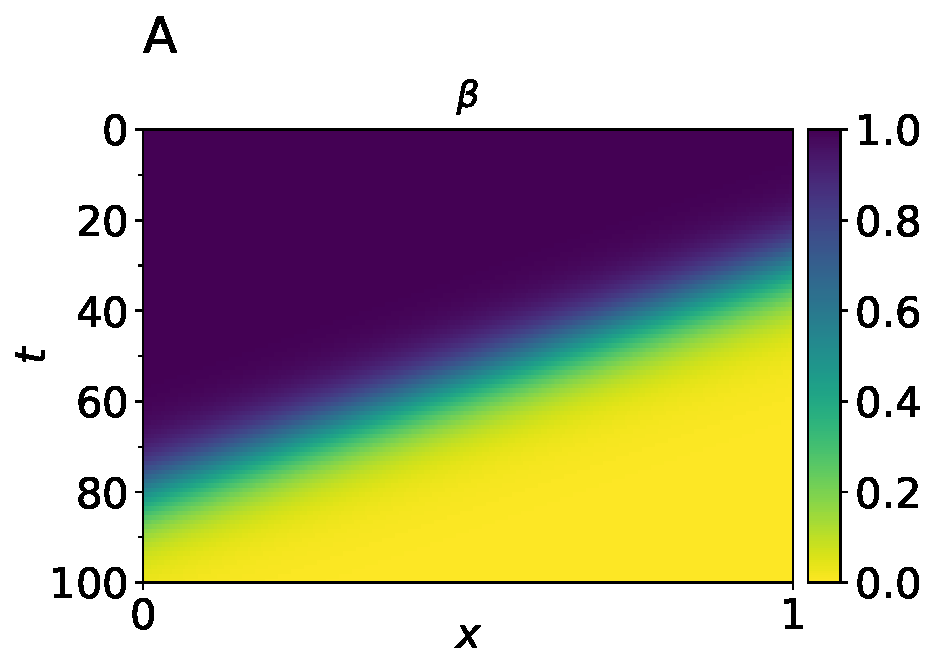
\includegraphics[width=2in]{Figures/Fig05aRev.pdf}
		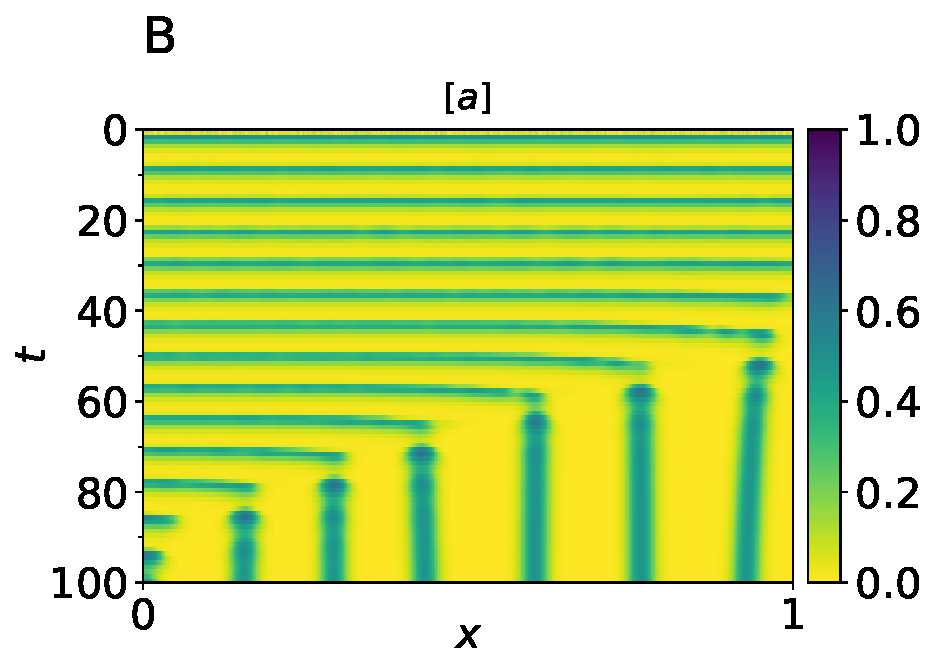
\includegraphics[width=2in]{Figures/Fig05bRev.pdf} 
		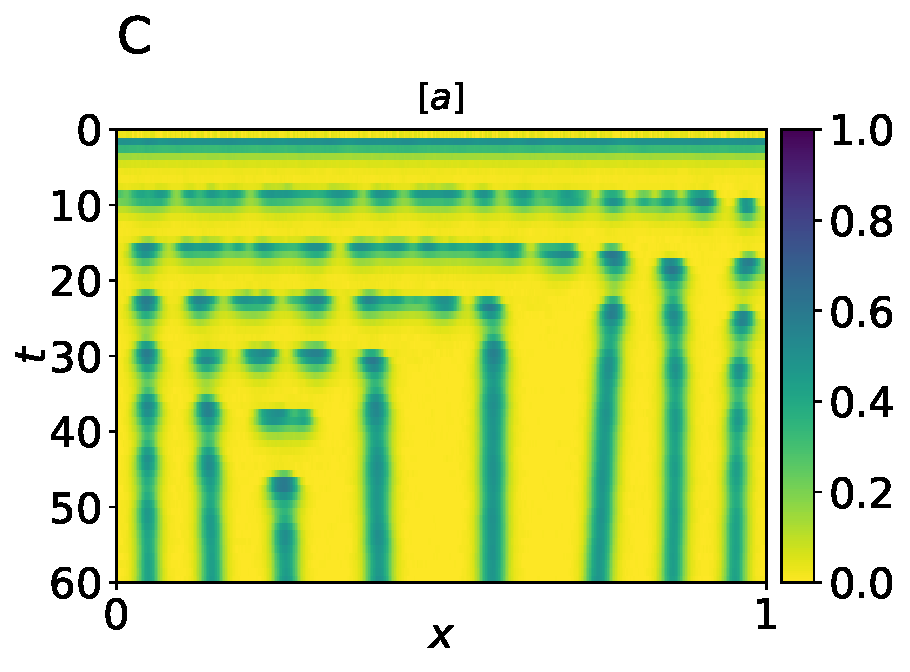
\includegraphics[width=2in]{Figures/Fig05cRev.pdf} 
		\caption{Spatio-temporal evolution of $a$ from system~\eqref{eq1112} for
			$\beta$-wave speed as in~\eqref{eqbeta}, with boundary condition as
			in~\eqref{eqbn}: (A)~$\beta$-wave evolution for speed $v=8$ for somite-pattern
			formation with noise intensity (B)~$c_v=0.05$ and (C)~$c_v=0.1$. Initial
			conditions for $A$ consists of random uniform distributions in the interval $[0,
			0.1]$, whereas $R(x, 0) = 0$ for all $x\in[0,1]$. Parameter values were set as
			follows: $k_1=0.05$, $k_2=0.01$, $k_3=2$, $n=3$,  $d_a = 5\times10^{-5}$
			and~$d_r=2.5\times10^{-3}$.}
		\label{Fig05}
	\end{figure}
	
	To summarize, the results presented in the paragraphs above confirm the
	hypothesis that a hybrid model, between the PORD and the clock-and-wavefront 
	models, undergoes a bifurcation from a stable to an 
	unstable limit cycle, as a result of its interaction with the
	wavefront, and
	that this bifurcation is enough to explain the observed robustness of
	somitogenesis and the independence on a specific initial condition. 
	To the best of our understanding, this hybrid model has
	a couple of quintessential features: it explains why somitogenesis may occur in the 
	absence of a wavefront (albeit in an irregular fashion), and how the process 
	achieves robustness as a consequence of the wavefront.
	
	
	\section{Concluding Remarks}
	\label{conclu}
	
	We have studied a hybrid model for somitogenesis, which incorporates 
	characteristics of the PORD (diffusion of the regulatory substances) and 
	clock-and-wavefront (the wavefront) models. By assuming that both the activator 
	and the repressor substances diffuse (the activator having a much smaller 
	diffusion coefficient), the model undergoes a bifurcation, from a stable to an 
	unstable limit cycle, as the value of the parameter accounting for the background
	regulatory input of the activator decreases. From a biological perspective, the
	bifurcation just described allows the model to explain why somites can form in
	the absence of a wavefront (which traditional front and wavefront models failed
	to explain), reassesses the role of the wavefront as a conductor for
	somitogenesis, and makes the model behavior robust to random fluctuations, as 
	well as independent from specific initial conditions;
	notice that the latter are two of the weak points of the original PORD model.  
	
	In the clock and wavefront models, there is a consensus that the oscillatory
	behavior is originated by a gene network with time-delayed negative feedback
	regulation \citep{Monk2003, Lewis2003}. This claim is supported by multiple
	experimental reports, which have elucidated some of the underlying regulatory
	mechanisms \citep{Schroter2012}. In contrast, the present and the
	\citet{Cotterell2015} models not only rely on a different gene network
	architecture to generate oscillations, but the genes in the network are
	hypothetical. From this perspective, the weight of experimental evidence seems
	to favor clock and wavefront models. Nonetheless, upon taking this into
	consideration, we
	believe that we have provided convincing evidence that reaction-diffusion and
	positional information (wavefront) mechanisms could work together in
	somitogenesis. Further investigating this possibility may allow a better
	understanding of such a fascinating phenomenon.
	
	
\section*{Acknowledgements}

JP-H thanks CONACYT-México for granting him a doctoral scholarship. VFBM thanks the financial support by Asociación Mexicana de Cultura AC. MS acknowledges the financial support of CONACYT-México, grant INFRA-302610. 
	
%	\pagebreak
	
	\appendix
	
%	\section{Bifurcation analysis of the diffusionless system}
	\section*{Appendix}
	\section{Somite pattern-formation dynamical features}
	\label{app:bif}
	\setcounter{equation}{0}
	\setcounter{figure}{0}    
	\renewcommand\thefigure{\thesection.\arabic{figure}}
	\renewcommand\theequation{\thesection.\arabic{equation}}
	System~\eqref{eq078910}, along with homogenous Neumann boundary conditions, gathers the essential ingredients of somite pattern-formation dynamics. Particularly, the kinetic terms consist of Hill functions, whose coefficients corresponding to a non-negative cooperative interaction. Thus, we assume that $n_3 = 1$ and $n_1 = n_2 = n\geq1$ as well as $\mu=1$. Initially, we set $d_a=d_r=0$. In so doing, we get the purely kinetic system:
	\begin{subequations}\label{eqA12}
		\begin{gather}\label{eqAR12}
		\frac{da}{dt}  = f(a,r)\,, \quad %\label{eqA1} \\[2mm]
		\dfrac{dr}{dt} = g(a,r)\,, %\label{eqA2}
		\end{gather}
		where the field components are given by
		\begin{gather}\label{eqnB034}
		f(a,r) = \dfrac{\beta + (a / k_1)^{n}}{1 + (a / k_1)^{n}
			+ (r / k_2)^{n}}-a\,, \quad g(a,r) = \dfrac{a}{k_3 + a}-r\,. 
		\end{gather}
	\end{subequations}
	This system steady states satisfy the relation $g(a)=\beta$, where
%	\begin{subequations}\label{eqA34}
%		\begin{gather}\label{eqA34}
%		a = \displaystyle \frac{\beta + (a / k_1)^{n}}{1 + (a / k_1)^{n} + (r /
%			k_2)^{n}}\,, \quad%\label{eqA3}  \\[2mm]
%		r = \frac{(a / k_3)}{1 + (a / k_3)}],. %\label{eqA4}
%		\end{gather}
%	\end{subequations}
%	If we take $f(a) := g(a)-\beta$ \\
%	with:
	\begin{gather}\label{eq:ga}
		g(a):=a-a^n/k_1^n+a^{n+1}/k_1^n +a\left(\frac{a/k_2}{k_3+a}\right)^n\,.
	\end{gather}
%	one solution for $f(a)$ meets that $g(a) = \beta$. That is, 
%	\begin{equation}
%	a-(a/k_1)^n+a^{n+1}/k_1^n +a\left(\frac{a/k_3}{k_2(1+a/k_3)}\right)^n =
%	\beta.
%	\end{equation}
	{From~\eqref{eq:ga}, notice that $g(a)$ satisfies that: (i)~$g(0) = 0$, and (ii)~$g(a)\rightarrow$ +$\infty$, when  $a\rightarrow +\infty$. In consequence, there exists $a^*>0$ such that $g(a^*) = \beta> 0 $, which further implies that $w^*=(a^*, r^*)$ is a steady-state of system~\eqref{eqA12}, with $a^* >0$ and $r^*>0$, since }
	\begin{gather*}
	r^* = \frac{a^*}{k_3+a^*}\,.
	\end{gather*}
	In other words, the existence of at least one steady-state in the first quadrant is guaranteed. We can straightforwardly  prove, from the Poincare-Bendixon theorem, that a limit-cycle family emerges as a result of this steady-state undergoing a Hopf bifurcation (HB). In order to disclose this implication, we performed a numerical continuation by using the algorithms implemented in XPPAUT (Ermentrout, 1987). The resulting bifurcation diagrams obtained by slowly varying each parameter of system~\eqref{eqA12} are depicted in Fig.~\ref{FigA01}. Notice that the system undergoes HBs for all parameters values in Table~\ref{Tab01}. In Fig.~\ref{FigA01}(a), a single HB for parameter $\beta$ takes place, where periodic orbits vanish at the bifurcation point HB. This suggests that the lower the $\beta$-input value, the larger the amplitude and the longer the period of stable orbits for the homogeneous system; and that no periodic orbits occur for $\beta\gg1$, nonetheless. In contrast, as is shown in Figs.~\ref{FigA01}(b)-(d), two supercritical HB points occur for parameters $k_1$, $k_2$ and $k_3$, which determine a finite interval for each parameter wherein a family of periodic orbits exist. Interestingly, a bi-stability interval for parameter $n$ is delimited by $n$-values where a subcritical HB and fold bifurcation (LP) points happen. That is, a branch consisting of unstable limit cycles emanates from the subcritical HB, which stabilizes at the LP points. Hence, stable steady-states coexist with stable limit-cycles for this interval, where the unstable periodic branch plays a critical role for initial states. This result, as is depicted in Fig.~\ref{FigA01}(e), indicates that an on-and-off gene switch is present, which provides hysteretical features triggered by key values of the characteristic Hill coefficient. We may argue from this that the cooperativity in the gene regulatory network favors system robustness to parameter variations.
	
	\begin{figure} %[t!]
		\centering
		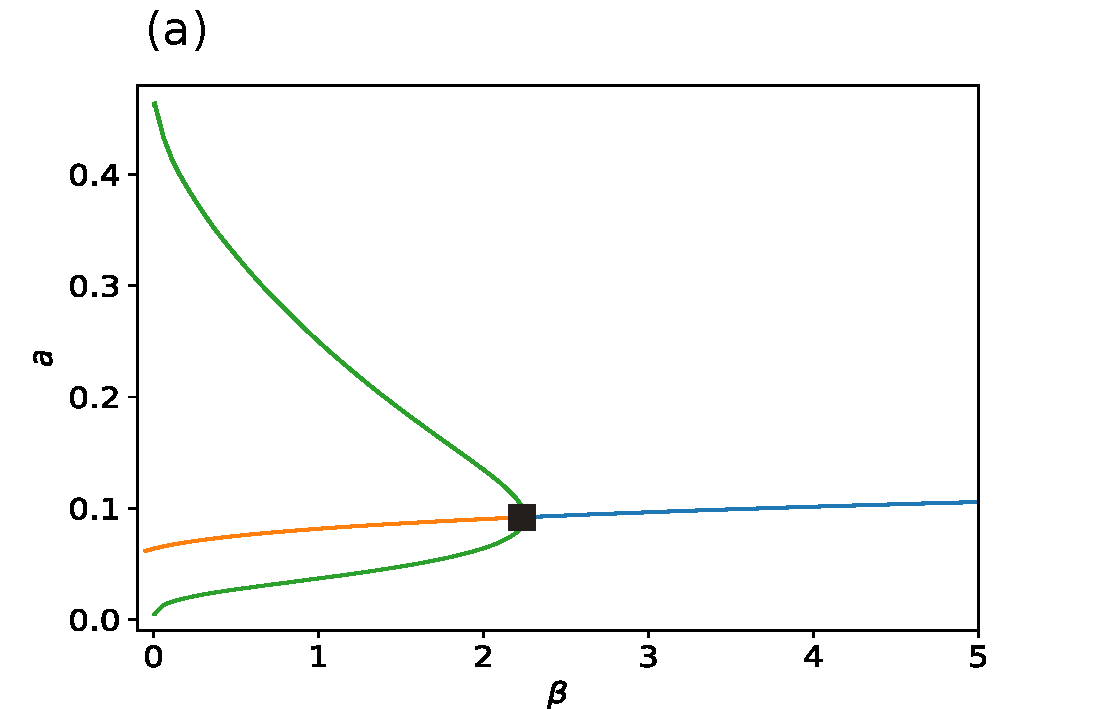
\includegraphics[width=3.8in]{Figures/ApFigure01a.pdf} \\
		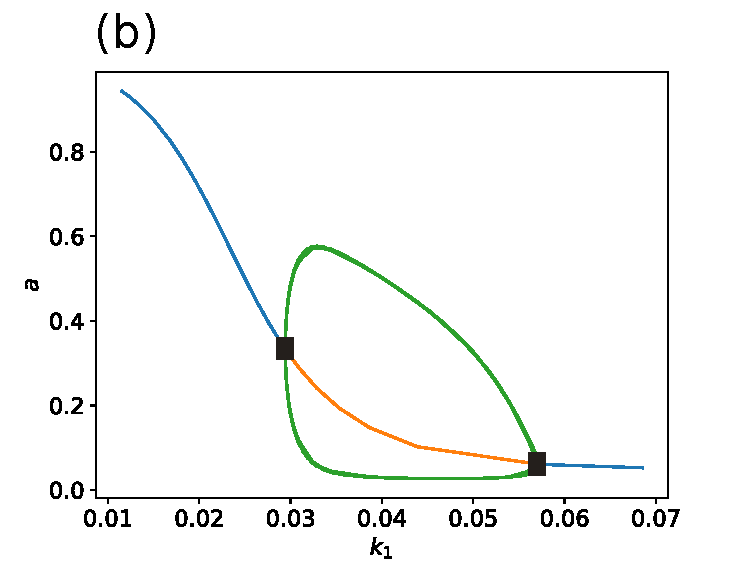
\includegraphics[width=2.8in]{Figures/ApFigure01b}
		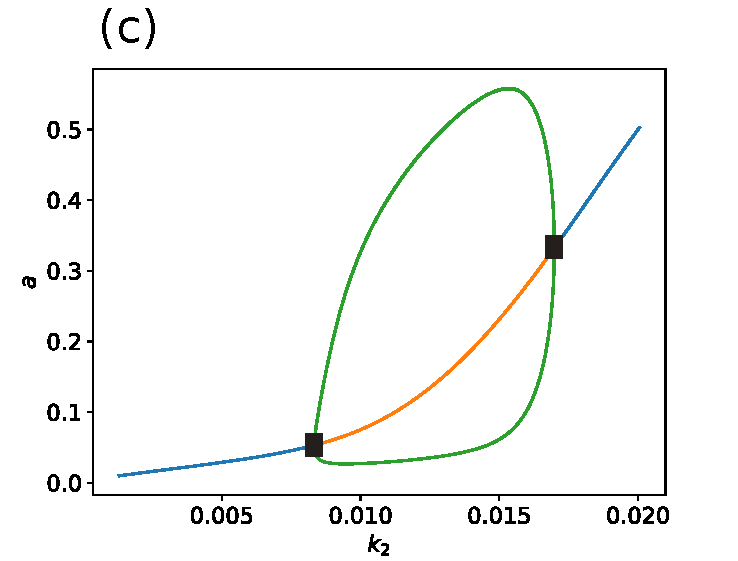
\includegraphics[width=2.9in]{Figures/ApFigure01c} \\
		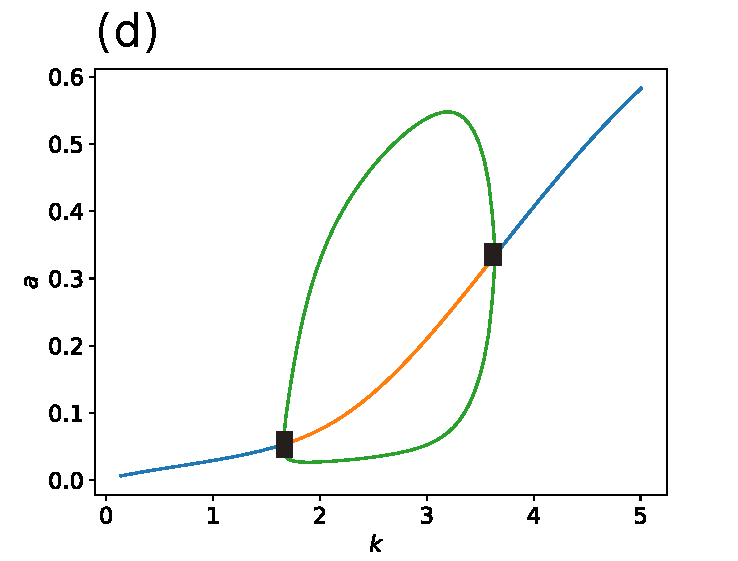
\includegraphics[width=2.8in]{Figures/ApFigure01d}
		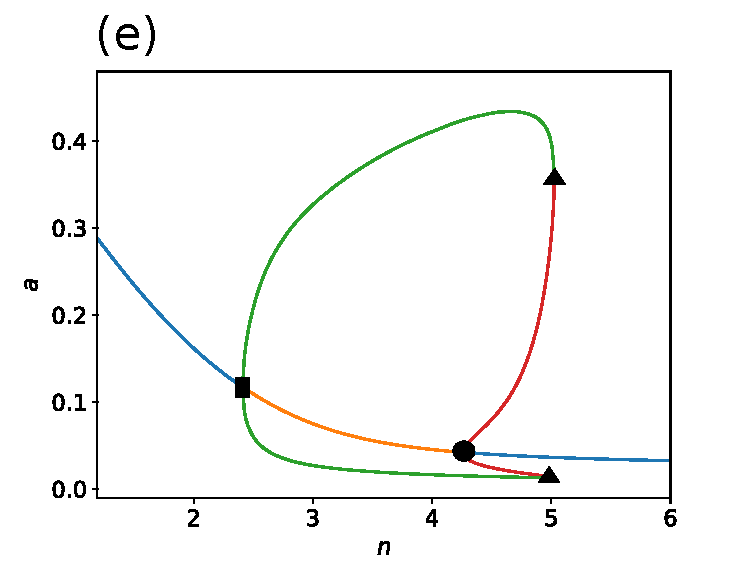
\includegraphics[width=3.0in]{Figures/ApFigure01e}
		\caption{Bifurcation diagrams of system~\eqref{eqA12} for slowly varying: (a)~background regulatory input of activator $\beta$,  effective half-saturation parameters (b)~$k_1$, (c)~$k_2$ and (d)~$k_3$, and (e)~Hill coefficient~$n$. Blue (orange) solid lines correspond to stable (unstable) branches of steady states, and green (red) lines are stable (unstable) limit-cycle branches. Squares (filled circle) indicate supercritical (subcritical) Hopf bifurcations, and triangle is for indicating fold bifurcations. Other parameter set values are $k_1 = 0.05$, $k_2 = 0.01$, $k_3 = 2.0$, $n=3.0$, and $\beta=0.5$, respectively.}
		\label{FigA01}
	\end{figure}
	
%\section{Spatial stability analysis}
%\label{app:stabil}
%	
%\setcounter{equation}{0}
%\setcounter{figure}{0}    
%\renewcommand\thefigure{\thesection.\arabic{figure}}
%\renewcommand\theequation{\thesection.\arabic{equation}}
	
On the other hand, as has been discussed above, the external regulation of gene $A$ is an essential ingredient of the somite pattern formation dynamics. Recall that this element is captured by $\beta$. In addition, the activator diffusion also plays a crucial role in the somite pattern-formation dynamics. We study now the interplay between $\beta$ and $d_a$, which triggers the somite formation mechanism that we have proposed. To do so, we include diffusion terms in~\eqref{eqA12} to get the reaction-diffusion system
%As before, we assume that $n_3 = \mu =1, n_2=n_1 = n$, and so rewrite the reaction-diffusion system~\eqref{eq078910} as follows:
%	\begin{subequations}
		\begin{gather}\label{eqnB01234}
		\frac{\partial{a}}{\partial{t}}= f(a,r)+d_a\nabla^2a\,, \quad \frac{\partial{r}}{\partial{t}} = g(a,r)+d_r\nabla^2r\,,%\label{eqnB01}\,,\\
%		\frac{\partial{r}}{\partial{t}} = g(a,r)+d_r\nabla^2r\,, \label{eqnB02}\,,
		\end{gather}
		where the kinetic terms are as in~\eqref{eqnB034}.
%		\begin{gather}\label{eqnB034}
%		f(a,r) = \dfrac{\beta + (r/k_1)^n}{1+(a/k_1)^n+(r/k_2)^n}-a\,, \quad g(a,r) = \dfrac{a/k_3}{1+a/k_3}-r\,. 
%		\end{gather}
%	\end{subequations}

Now, upon defining $w=(a,r)^T$, we obtain that system~\eqref{eqnB01234} can be set up in vector notation as $w_t = F(w) + D \nabla^2 w$, where
%	\begin{gather}\label{eqvector}
%	w_t = F(w) + D \nabla^2 w\,, 
%	\end{gather}
	$F(w) = \left(f(a,r),g(a,r)\right)^T$ and $D=\textrm{diag}\left(d_a, d_r \right)$. In so doing, for an isolated root of $F(w)=0$ given by $w^*=(a^*,r^*)$, system~\eqref{eqnB01234} has a local solution of the form  
	\begin{gather}\label{eqnB06}
	w(x,t)= \sum_{m=0}^{\infty}\gamma_me^{-\lambda\left(\kappa^2\right) t}w_m(x)\,,%\cos(\kappa x)\,,
	\end{gather}
	where $w_m(x)$ satisfies the Helmholtz equation $\nabla^2w_m+\kappa^2w_m=0$, in which the so-called wave mode is denoted by $\kappa$. The Fourier coefficients $\gamma_m$ are determined by the initial conditions, and $\lambda$ determines whether~\eqref{eqnB06} converges, and hence is bounded, as $t\to+\infty$. These three parameters not only shape solution~\eqref{eqnB06}, but also are intrinsic to the geometry and boundary conditions of the system into consideration. Moreover, they also depend on the wave number $m\in\mathbb{N}$; see~\citep{Murray1989} for further details. 

We now derive the dispersion relation, which gives a linear insight of solution features depending on the parameters. To do so, we linearize system~\eqref{eqnB01234} at $w^*$ to get, in vectorial form,
	\begin{gather}\label{eqnB07}
	w_t = Jw + D \nabla^2 w	\,,
	\end{gather}
	where $J$ is the Jacobian matrix at $w^*$. Now, as our interest lies on the dynamics in one spatial dimension, we have that $w_m(x)=\cos(\kappa x)$, where $\kappa=m\pi/L$ satisfies the Helmholtz equation for homogenous Neumann boundary conditions as in~\eqref{eqbn}. Thus, \eqref{eqnB07} is satisfied by~\eqref{eqnB06}, when the dispersion relation $\lambda=\lambda(\kappa)$ is given by
	\begin{gather}\label{eqnB13}
	|J-D\kappa^2-\lambda I|=0\,, \quad I\in\mathbb{R}^{2\times2}\,,
	\end{gather}
	which can be seen by substituting~\eqref{eqnB06} into~\eqref{eqnB07}. As a result, it relates the temporal growth rate and the spatial wave mode $\kappa$, which parametrises the finite spatial domain. Note that~\eqref{eqnB13} leads to 
	\begin{subequations}\label{eq:lambda}
		\begin{gather}\label{eqnB14}
		\lambda^2 + b(\kappa^2)\lambda + c(\kappa^2) =0\,,
		\end{gather}
		where
		\begin{flalign}
		& b(\kappa^2)=(d_a+d_r)\kappa^2 -(f_a+g_r)\,, \label{eqnB15} \\
		& c(\kappa^2)=d_ad_r\kappa^4-(d_rf_a+d_ag_r)\kappa^2+ (f_ag_r-f_rg_a) \,.\label{eqnB16}
		\end{flalign}
	\end{subequations}
As we are interested in the linear stability of the steady state $w^*$, characterized by parameters~$\beta$~and~$d_a$, we notice that the parameter space for spatial instability of Turing type is given by conditions: 
\begin{subequations} \label{eqnB17}
	\begin{gather}
	f_a+g_r<0\,, \quad f_ag_v-f_rg_a>0 \,, \label{eqnB18} \\
	d_rf_a + d_ag_r > 0 \,, \quad d_rf_a + d_ag_r > 2\sqrt{d_ad_r(f_ag_r-f_rg_a)} \,. \label{eqnB20}%\label{eqnB19} \\
%	d_rf_a + d_ag_r > 2\sqrt{d_ad_r(f_ag_r-f_rg_a)} \,. \label{eqnB20}
	\end{gather}
\end{subequations} 
These conditions provide the ingredients that give place to non homogeneous spatially extended stationary states. We are however interested in a mechanism that triggers sustained oscillations of the gene network that give place to a stationary pattern in the long term. Such a process is dynamically provided by the Turing-Hopf bifurcation (THB); see, for instance,~\citep{Castillo2016, liu}. From~\eqref{eqnB14}, this bifurcation is prompted by obtaining purely imaginary eigenvalues by slowly varying $d_a$ or $\beta$. In so doing, we notice that two key conditions must be met: (i)~$f_a + g_r=0$ at the THB point, and (ii)~$d\lambda(\kappa^2;p^*)/dp\neq0$, also known as transversality condition, where $p^*=d_a^*$ or $p^*=\beta^*$ represent the THB parameter value. Thus, in order to obtain the parameter regions where a Turing bifurcation, HB and THB occur in system~\eqref{eqnB01234}, we solve~\eqref{eq:lambda} for $\lambda(\kappa^2)$. In Fig.~\ref{FigB01}, the parameter space on scope is portrayed, where four different stability features for the selected range values of parameters $\beta$ and $d_a$ are identified in four regions, labeled accordingly: Turing pattern, Turing-Hopf pattern, Hopf pattern, and no pattern. Notice that, at the transition curve between region II and III, parameters $\beta$ and $d_a$ follow an inverse relation; in other words, the larger parameter $\beta$ is, the lower diffusivity $d_a$ is needed for the bifurcation to take place. In addition, notice that for a fixed value of $d_a=5\times10^{-5}$, slowly varying $\beta$ from 0 up to 1 drives the system through two bifurcations, which in turn originate three different mechanisms. That is, no pattern is formed for $0\leq\beta < 0.5\times10^{-2}$, which is followed by getting into the Turing-Hopf pattern region for $ 0.5\times10^{-2}<\beta<0.5$, to get in the Hopf pattern region, which is held by $ 0.5<\beta\leq 1.0$. 

\begin{figure}[t!]
	\centering
	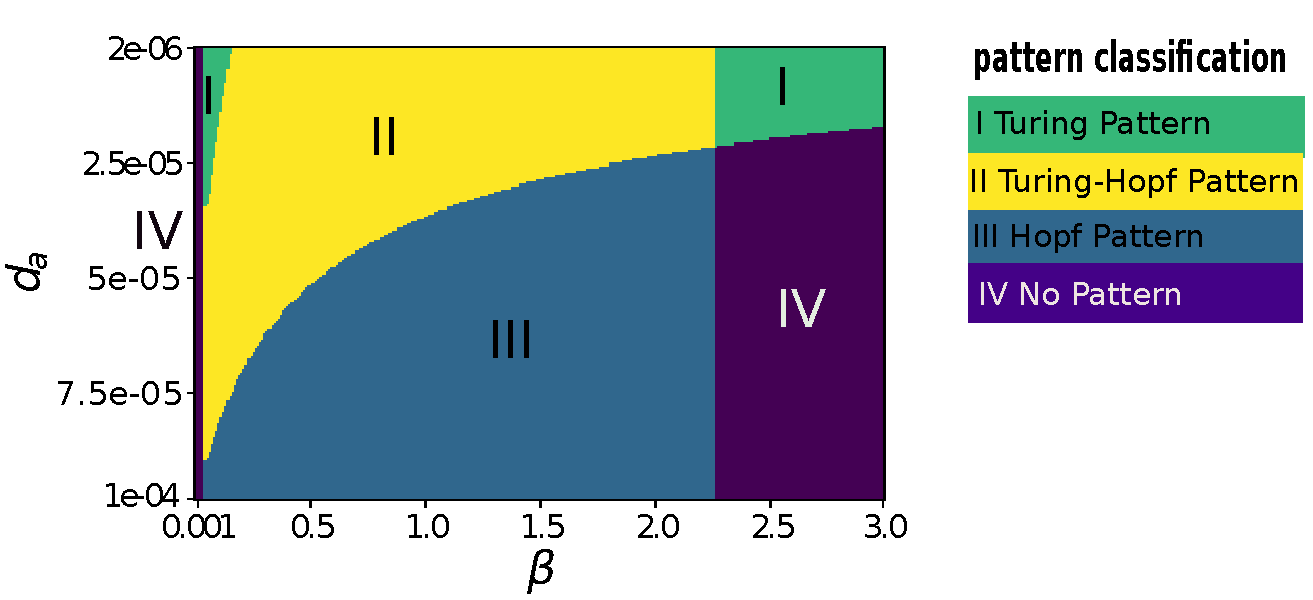
\includegraphics[width=5.0in]{Figures/ApFigure01}
	\caption{Two-parameter space for $d_a$ and $\beta$. Each pattern region is plotted in colors accordingly to the table in the right-hand side, and transition lines correspond to each region boundary. Other parameter set values are $d_r = 2.5\times10^{-3}, k_1 = 5\times10^{-2}, k_2=10^{-2}, k_3=2.0, n=3.0$.}
	\label{FigB01}
\end{figure}

\begin{figure}[t!]
	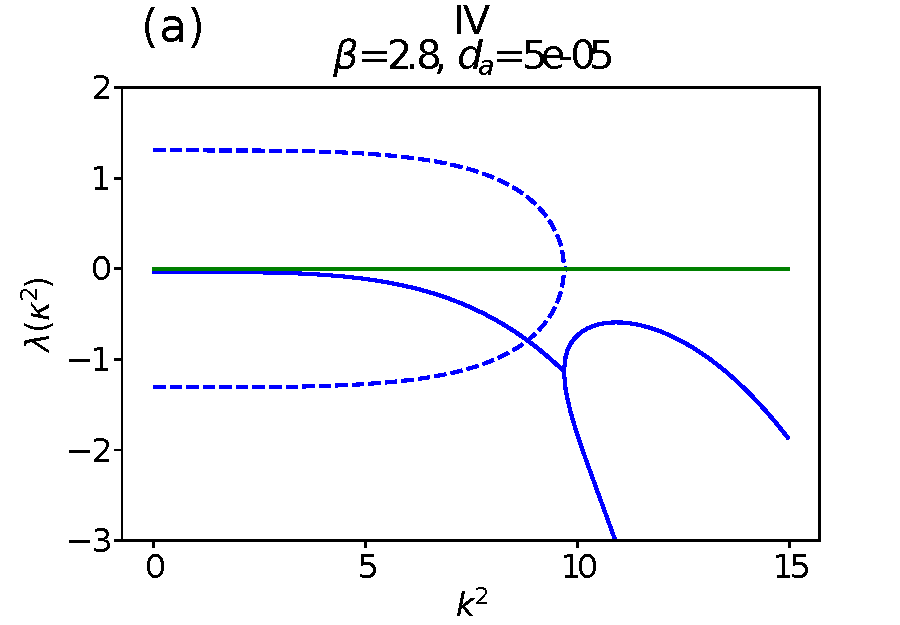
\includegraphics[width=3.2in]{Figures/ApFigure02a} 
	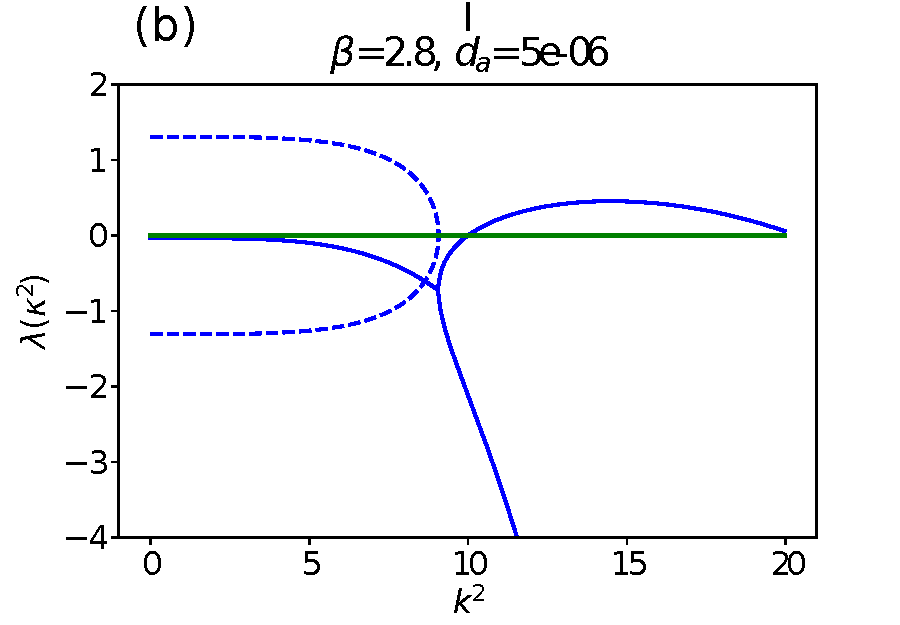
\includegraphics[width=3.2in]{Figures/ApFigure02b}\\
	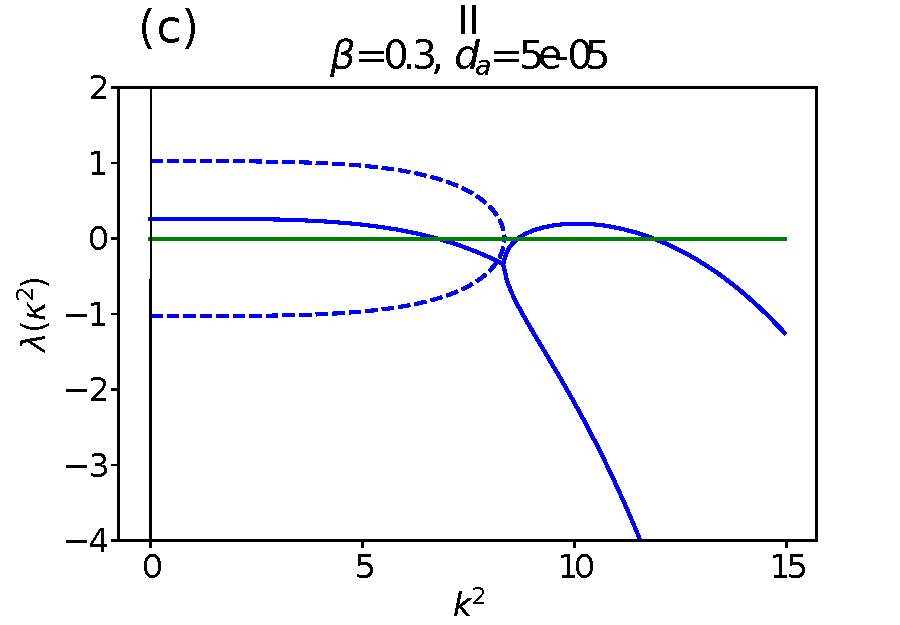
\includegraphics[width=3.2in]{Figures/ApFigure02c} 
	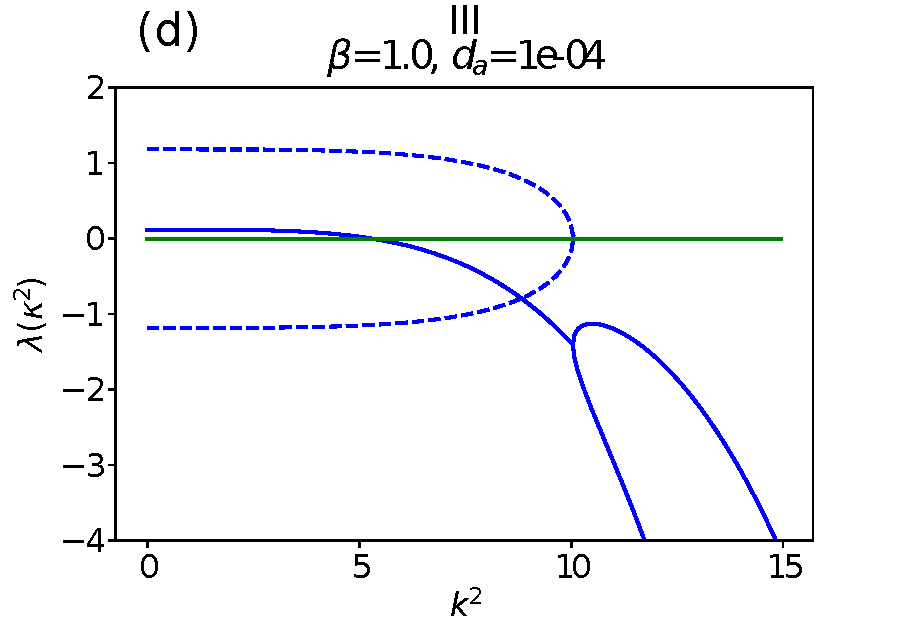
\includegraphics[width=3.2in]{Figures/ApFigure02d} 
	\caption{Samples of dispersion relations for each region depicted in Fig.~\ref{FigB01}. The real parts of the eigenvalues are in solid lines, and the imaginary parts in dashed lines.  Panel (a) corresponds to region IV, where the real part is negative for all $\kappa^2$; in panel (b) the real part has two roots, which gives place to a Turing type stationary pattern; in panel (c), Turing and Hopf bifurcations occur for different wave modes: the real part line is positive for wave modes corresponding to non-zero imaginary part, and a Turing instability occurs as in panel (b); in  panel (d), a typical Hopf bifurcation feature is exhibited as the real part is positive only for non-zero portions of the imaginary part. The values of $d_a$ and $\beta$ are respectively shown in each panel, and other parameters values are $k_1=5\times10^{-2}, k_2=10^{-2}, k_3=2.0, n=3.0$.}
	\label{FigB02}
\end{figure}

The four kinds of patterns depicted in Fig.~\ref{FigB01} are classified according to the roots of~\eqref{eq:lambda}. A sample of each root-solution type is plotted in Fig \ref{FigB02}, where solid lines are  the real part of the eigenvalues and the dashed lines correspond to the imaginary part. The Turing pattern region is labelled by I; as can be seen there, the dispersion relation has a finite positive maximum which gives place to an interval of unstable wave modes. For region II, a Turing-Hopf pattern dispersion relation is depicted, where the imaginary part is non zero for positive portions of the real part, and when the imaginary part colapses to zero, the real part is as in the Turing region. That is, this stability feature gathers two main dynamical ingredients: oscillatory and non oscillatory unstable modes in two finite disconected subintervals. In region III, a Hopf pattern is characterized by having a dispersion relation in which the real part is only non negative for wave modes where the imaginary part is non zero. Finally, region IV corresponds to no pattern, which is characterized by having a negative real part of the dispersion relation for all wave modes, and hence the homogeneous steady state suffers no symmetry breaking. In other words, the combination of real and imaginary parts of $\lambda(\kappa^2)$ in~\eqref{eqnB06}, and provided by~\eqref{eqnB13}, determines each pattern type as well as transitions between regions. For a detailed discussion about the former approach, see~\citep{liu}.

\begin{figure}[t!]
 		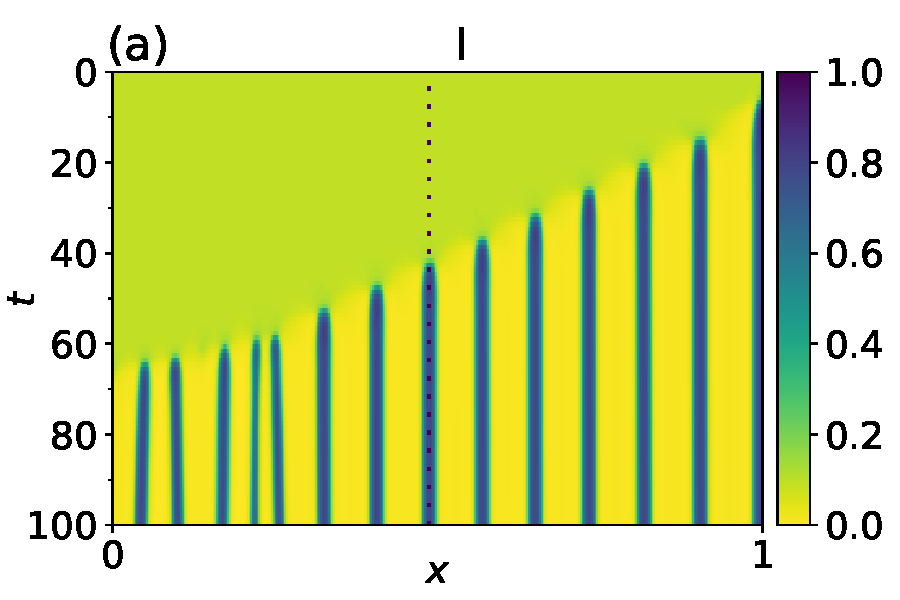
\includegraphics[width=3.2in]{Figures/ApFigure03a}
		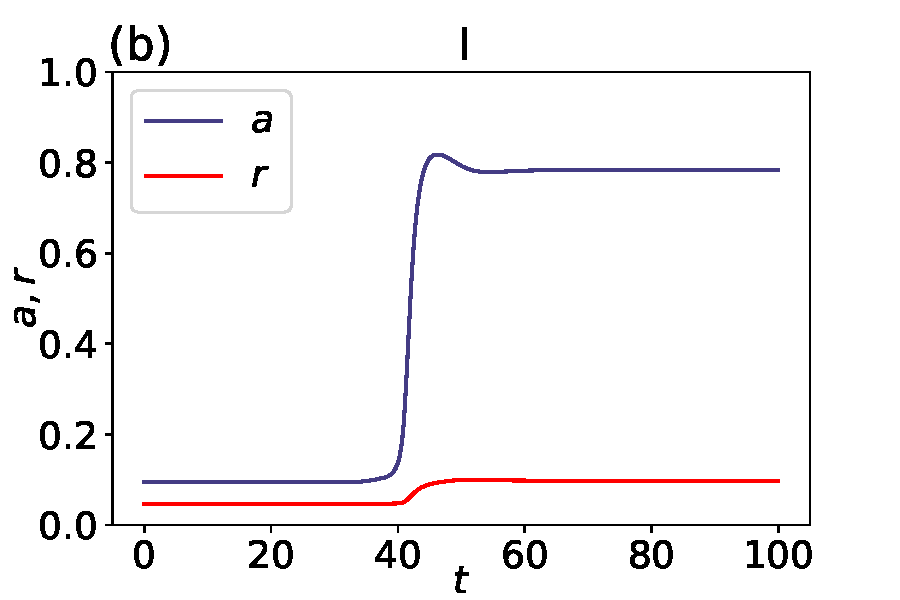
\includegraphics[width=3.2in]{Figures/ApFigure03b}\\
		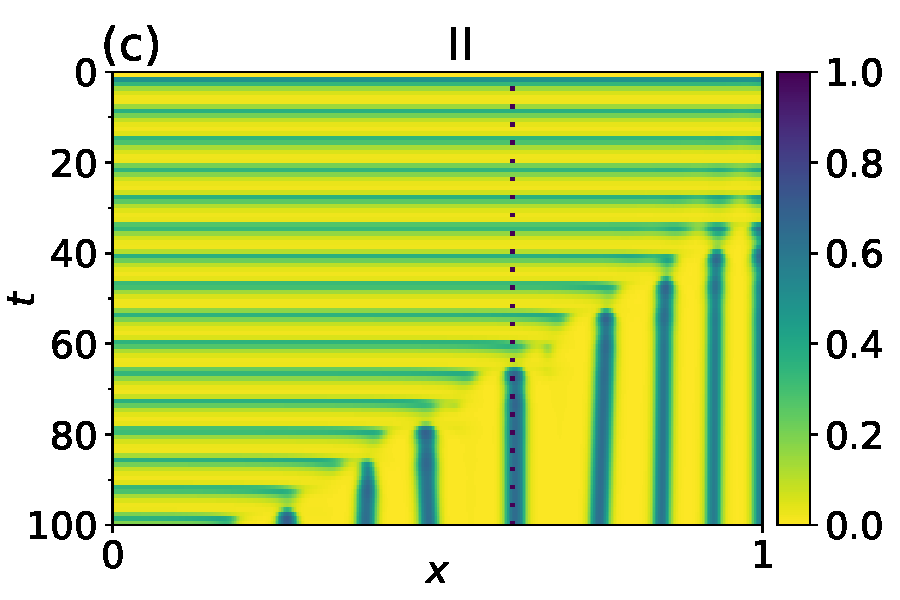
\includegraphics[width=3.2in]{Figures/ApFigure03c}
		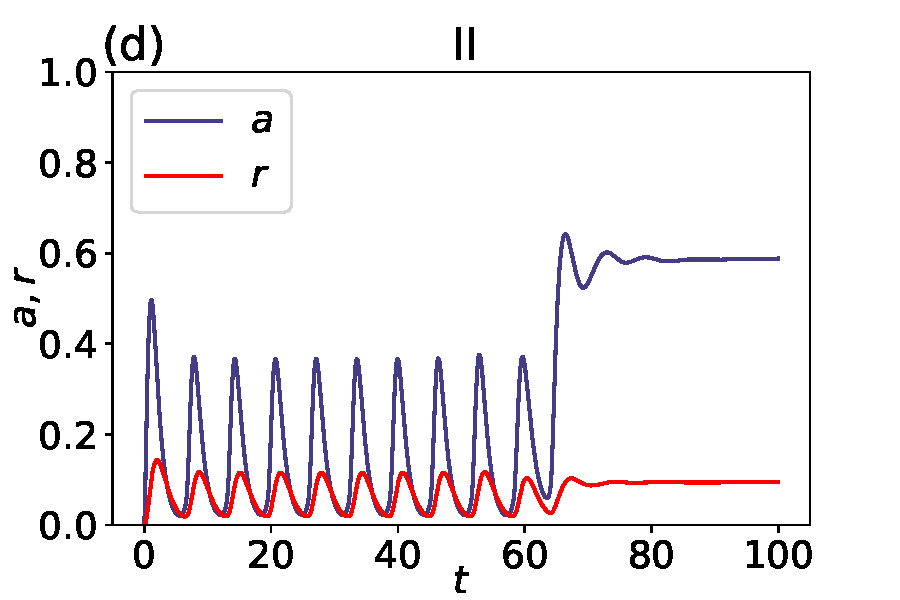
\includegraphics[width=3.2in]{Figures/ApFigure03d}\\
		\caption{Time-step simulations of~\eqref{eqnB01234} with homogeneous Neumann boundary conditions and parameter set values as in region I and II plotted in~Fig.~\ref{FigB01}. An azimuthal view of the spatio-temporal solution shows the pattern formation dynamics for a Turing type (panel a) and a Turing-Hopf type (panel c). Temporal evolution for each case in the left-hand side column of the activator and repressor at $x=0.6125$ and $x=0.4875$ (dashed lines in panels a and c) are shown in panels (b) and (d), respectively. Initial conditions were taken as a perturbation of the steady state accordingly to regions~I~and~II, respectively, of the parameter space in Fig.~\ref{FigB01}.}
		\label{FigB03}
	\end{figure}
	
	\begin{figure}%[t!]
		\centering
		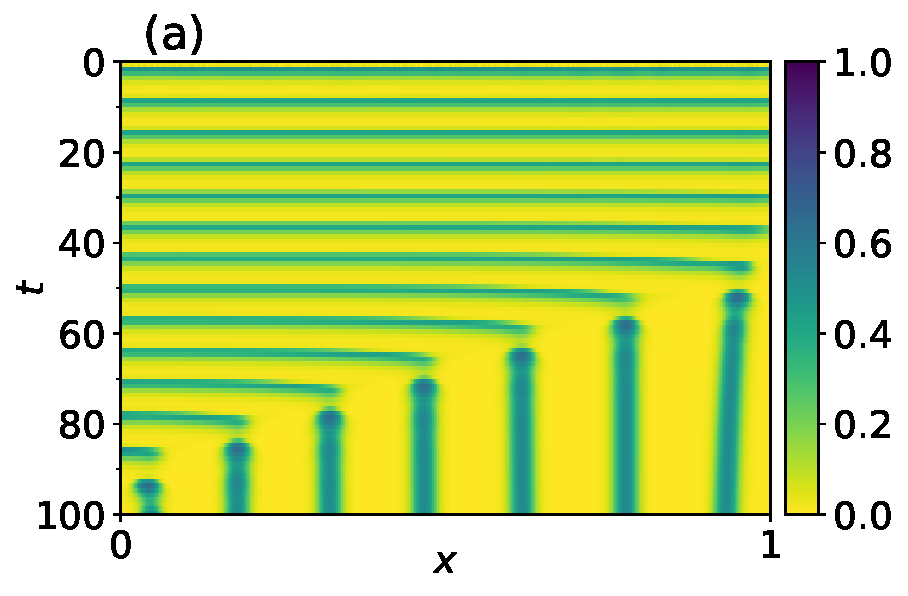
\includegraphics[width=3.2in]{Figures/ApFigure04a}
		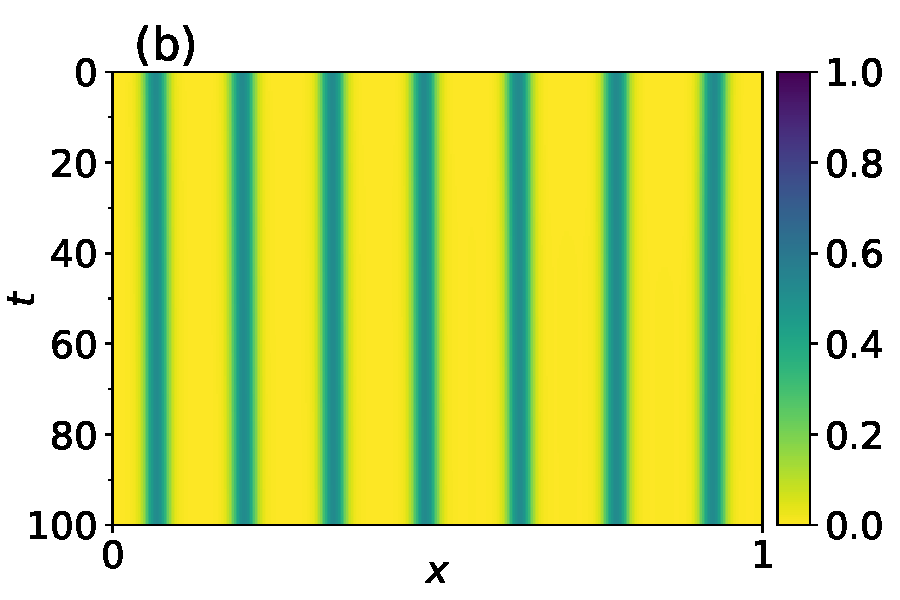
\includegraphics[width=3.2in]{Figures/ApFigure04b}
		%\includegraphics[width=3.2in]{Figures/ApFigure04c}
		%\includegraphics[width=3.2in]{Figures/ApFigure04d}
		\caption{Simulations with parameter $\beta$ as function of $x$ and $t$ as indicated in the text. For (a), the initial conditions are perturbations of the steady state,
		while in (b) the initial conditions are the final state of (a).}
		\label{FigB04}
	\end{figure}

Regions I and II are particularly relevant as a stationary pattern is formed, although a key mark lies on transitory dynamical behavior for each scenario. To illustrate this distinguished mark, we perform time-step runs for a setting in both regions, by having a perturbed steady state as an initial condition; see top panels in Fig.~\ref{FigB03}. As can be seen in panel (a), the system is initially in a homogeneous steady state with a slight perturbation. As time goes by, a heterogeneous pattern arises. This is a consequence of the unstable wave modes as is shown in~Fig.~\ref{FigB02}, panel (b), which corresponds to the Turing pattern, region I, in Fig.~\ref{FigB01}. In addition, in panel (b), a time evolution is observed for the activator and repressor states at $x=0.6125$. On the other hand, in an analogous fashion, the transitory dynamics spontaneously oscillate as a consequence of the non zero imaginary part of $\lambda(\kappa^2)$. Such oscillatory dynamics goes on until unstable wave modes allow a stationary pattern to arise. Notice that this mark is clearly observed in panel (d); see bottom panels in Fig.~\ref{FigB03}. In other words, even though both dynamical configurations give place to stationary patterns, the crucial oscillating feature previous to finally get a fixed pattern is added by having a Turing-Hopf mechanism in play.
	
In Fig \ref{FigB04}, we show additional results, where a spatio-temporal dependent parameter $\beta$ is taken into consideration. There, we take $\beta$ as in (\ref{eqbeta}) %a decreasing function of $x$ and $t$, %namely
%	\begin{gather}\label{eq:betaxt}
%		\beta(x,t) = \dfrac{\beta_0 k^n}{k^n+(xv(t))^n}\,,
%	\end{gather}
where $v=0.02$ and $v=-0.02$ for the run in panels (a) and (b), respectively. The initial conditions for panel (b) corresponds to the final profile of panel (a). Notice that once the pattern is completely formed, even though $\beta$ varies in a inverse direction, the pattern is not destroyed. This is typical trait of a hysteretical process. In other words, this result indicates that the proposed mechanism is robust since, once the wave front depicted by $\beta$ in (\ref{eqbeta}) prompts the formation of somites, this process cannot be undo.

\clearpage

\bibliography{ReactionDiffusion}

\end{document}

	\begin{gather}\label{eqbn}
	\left. \dfrac{\partial a}{\partial x}\right|_{(0, t)} = 
	\left. \dfrac{\partial a}{\partial x}\right|_{(1, t)} = 
	\left. \dfrac{\partial r}{\partial x}\right|_{(0, t)} =
	\left. \dfrac{\partial r}{\partial x}\right|_{(1, t)} = 0 ,
	\end{gather}
	with, unless otherwise stated, the following initial conditions: 
	\begin{gather}
	a(x, 0) = \left\{\begin{array}{cl}
	0.05 & \text{for } x = 1, \\
	0 & \text{for } 0 \leq x < 1,
	\end{array} \right. 
	\quad
	r(x, 0) = 0, \; \text{for } 0 \leq x \leq 1\,.
	\end{gather}
	That is, the system is assumed to be initially homogeneous, except for a
	perturbation at the anterior extreme of the observation window.
